\lhead{CLRS {--} Chapter 6 {--} Heapsort}

{\large Section 6.1 {--} Heaps}

\begin{enumerate}

\item[6.1{-}1]{What are the minimum and maximum numbers of elements in a heap of
height $h$?}

\begin{framed}
Minimum is $2^{h}$. Maximum is $2^{h + 1} - 1$.
\end{framed}

\item[6.1{-}2]{Show that an $n$-element heap has height $\floor{\lg n}$.}

\begin{framed}
A heap of height $h + 1$ is a complete tree of height $h$ plus one additional
level with $1 \le k \le 2^h$ nodes. This additional level does not count to the
height of the heap, which then explain the height of $\floor{\lg n}$.
\end{framed}

\item[6.1{-}3]{Show that in any subtree of a max-heap, the root of the subtree
contains the largest value occurring anywhere in that subtree.}

\begin{framed}
  Every node of the subtree has a path upwards to the root of the subtree.
  Therefore, the max-heap property assures that each of these nodes are no
  larger than the root of the subtree.
\end{framed}

\item[6.1{-}4]{Where in a max-heap might the smallest element reside, assuming
that all elements are distinct?}

\begin{framed}
In the leaves. Note that, since the bottom level may be incomplete, in addition
to the nodes on level zero, some of the nodes on level one may also be leaves.
\end{framed}

\item[6.1{-}5]{Is an array that is in sorted order a min-heap?}

\begin{framed}
Yes, since for each node $i$, we have $A[\textsc{Parent}(i)] \le A[i]$.
\end{framed}

\item[6.1{-}6]{Is the array with values
$\langle 23, 17, 14, 6, 13, 10, 1, 5, 7, 12 \rangle$ a max-heap?}

\begin{framed}
No. The element 6 is the parent of the element 7 and $6 < 7$, which violates the
min-heap property.
\end{framed}

\item[6.1{-}7]{Show that, with the array representation for storing an
$n$-element heap, the leaves are the nodes indexed by
$\floor{n/2} + 1, \ceil{n/2} + 2, \dots, n$.}

\begin{framed}
The parent of the last element of the array is the element at position
$\floor{n/2}$, which implies that all elements after $\floor{n/2}$ has no
children and are therefore leaves. Also, since the element at position
$\floor{n/2}$ has at least one child (the element at position $n$), the
elements before $\floor{n/2}$ also have and therefore can not be leaves.
\end{framed}

\end{enumerate}

\newpage

{\large Section 6.2 {--} Maintaining the heap property}

\begin{enumerate}

\item[6.2-1]{Using Figure 6.2 as a model, illustrate the operation of
\textsc{Max-Heapify}$(A, 3)$ on the array
$A = \langle 27, 17, 3, 16, 13, 10, 1, 5, 7, 12, 4, 8, 9, 0 \rangle$.}

\begin{framed}
\begin{center}
\begin{tikzpicture}
\Tree
[.27
    [.17
    \edge[];
        [.16
        \edge[]; {5}
        \edge[]; {7}
        ]
    \edge[];
        [.13
        \edge[]; {12}
        \edge[]; {4}
        ]
    ]
    [.\node[red]{3};
    \edge[red];
        [.\node[red]{10};
        \edge[]; {8}
        \edge[]; {9}
        ]
    \edge[];
        [.1
        \edge[]; {0}
        \edge[blank]; \node[blank]{};
        ]
    ]
]
\end{tikzpicture}
\begin{tikzpicture}
\Tree
[.27
    [.17
    \edge[];
        [.16
        \edge[]; {5}
        \edge[]; {7}
        ]
    \edge[];
        [.13
        \edge[]; {12}
        \edge[]; {4}
        ]
    ]
    [.10
    \edge[];
        [.\node[red]{3};
        \edge[]; {8}
        \edge[red]; \node[red]{9};
        ]
    \edge[];
        [.1
        \edge[]; {0}
        \edge[blank]; \node[blank]{};
        ]
    ]
]
\end{tikzpicture}
\begin{tikzpicture}
\Tree
[.27
    [.17
    \edge[];
        [.16
        \edge[]; {5}
        \edge[]; {7}
        ]
    \edge[];
        [.13
        \edge[]; {12}
        \edge[]; {4}
        ]
    ]
    [.10
    \edge[];
        [.9
        \edge[]; {8}
        \edge[]; {3}
        ]
    \edge[];
        [.1
        \edge[]; {0}
        \edge[blank]; \node[blank]{};
        ]
    ]
]
\end{tikzpicture}
\end{center}
\end{framed}

\item[6.2-2]{Starting with the procedure \textsc{Max-Heapify}, write pseudocode
for the procedure \textsc{Min-Heapify}$(A, i)$, which performs the corresponding
manipulation on a min-heap. How does the running time of \textsc{Min-Heapify}
compare to that of \textsc{Max-Heapify}?}

\begin{framed}
The pseudocode is stated below.

\begin{algorithm}[H]
\SetAlgoNoEnd\DontPrintSemicolon
\BlankLine
\SetKwFunction{algo}{Min-Heapify}
\SetKwProg{myalg}{}{}{}
\myalg{\algo{A, i}}{%
\nl $l = \texttt{Left}(i)$\;
\nl $r = \texttt{Right}(i)$\;
\nl \If{$l \le A.\text{\emph{heap-size}}$ \upshape{and} $A[l] < A[i]$}{%
\nl   $\text{\emph{smallest}} = l$\; }
\nl \Else{%
\nl   $\text{\emph{smallest}} = i$\; }
\nl \If{$r \le A.\text{\emph{heap-size}}$ \upshape{and} $A[r] < A[smallest]$}{%
\nl   $\text{\emph{smallest}} = r$\;}
\nl \If{$\text{\emph{smallest}} \neq i$}{%
\nl   \upshape{exchange} $A[i]$ \upshape{with} $A[smallest]$\;
\nl   \texttt{Min-Heapify}$(A, \text{\emph{smallest}})$\; } }
\end{algorithm}

The running time is the same.
\end{framed}

\item[6.2-3]{What is the effect of calling \textsc{Max-Heapify}$(A, i)$ when the
element $A[i]$ is larger than its children?}

\begin{framed}
Node $i$ and its children already satisfies the max-heap property. No recursion
will be called and the array will keep the same.
\end{framed}

\item[6.2-4]{What is the effect of calling \textsc{Max-Heapify}$(A, i)$ for
$i > A.\text{\emph{heap-size}}/2$?}

\begin{framed}
Every node $i > A.\text{\emph{heap-size}}/2$ is a leaf. No recursion will be
called and the array will keep the same.
\end{framed}

\newpage

\item[6.2-5]{The code for \textsc{Max-Heapify} is quite efficient in terms of
constant factors, except possibly for the recursive call in line 10, which might
cause some compilers to produce inefficient code. Write an efficient
\textsc{Max-Heapify} that uses an iterative control construct (a loop) instead
of recursion.}

\begin{framed}
The pseudocode is stated below.

\begin{algorithm}[H]
\SetAlgoNoEnd\DontPrintSemicolon
\BlankLine
\SetKwFunction{algo}{Max-Heapify-Iterative}
\SetKwProg{myalg}{}{}{}
\myalg{\algo{A, i}}{%
\nl $\text{\emph{solved}} = \texttt{False}$\;
\nl $\text{\emph{current-node}} = i$\;
\nl \While{\upshape{not} \text{\emph{solved}}}{%
\nl   $l = \texttt{Left}(\text{\emph{current-node}})$\;
\nl   $r = \texttt{Right}(\text{\emph{current-node}})$\;
\nl   \If{$l \le A.\text{heap-size}$ \upshape{and} $A[l] > A[\text{\emph{current-node}}]$}{%
\nl     $\text{\emph{largest}} = l$\; }
\nl   \Else{%
\nl     $\text{\emph{largest}} = \text{\emph{current-node}}$\; }
\nl   \If{$r \le A.\text{heap-size}$ \upshape{and} $A[r] > A[\text{\emph{largest}}]$}{%
\nl     $\text{\emph{largest}} = r$\;}
\nl   \If{$\text{largest} \neq \text{current-node}$}{%
\nl     \upshape{exchange} $A[\text{\emph{current-node}}]$ \upshape{with} $A[\text{\emph{largest}}]$\;
\nl     $\text{\emph{current-node}} = \text{\emph{largest}}$\; }
\nl   \Else{%
\nl     $\text{\emph{solved}} = \texttt{True}$\; } } }
\end{algorithm}
\end{framed}

\item[6.2-6]{Show that the worst-case running time of \textsc{Max-Heapify} on a
heap of size $n$ is $\Omega(\lg n)$. (Hint: For a heap with $n$ nodes, give node
values that cause \textsc{Max-Heapify} to be called recursively at every node on
a simple path from the root down to a leaf.)}

\begin{framed}
The worst-case occurs when $A[\textsc{Left}(i)] \ge A[\textsc{Right}(i)] > A[i]$
in each level of the recursion, which will cause the node to be pushed to the
leftmost position on the bottom level of the heap. There will be exactly
$\floor{\lg n}$ recursive calls (in addition to the first call). Since each call
is $\Theta(1)$, the total running time is
$\floor{\lg n} \cdot \Theta(1) = \Theta(\lg n) = \Omega(\lg n)$.
\end{framed}

\end{enumerate}

\newpage

{\large Section 6.3 {--} Building a heap}

\begin{enumerate}

\item[6.3-1]{Using Figure 6.3 as a model, illustrate the operation of
\textsc{Build-Max-Heap} on the array
$A = \langle 5, 3, 17, 10, 84, 19, 6, 22, 9 \rangle$.}

\begin{framed}
\begin{center}
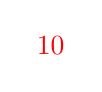
\begin{tikzpicture}
\Tree
[.5
    [.3
    \edge[];
        [.\node[red]{10};
        \edge[]; {22}
        \edge[]; {9}
        ]
    \edge[]; {84}
    ]
    [.17
    \edge[]; {19}
    \edge[]; {6}
    ]
]
\end{tikzpicture}
\begin{tikzpicture}
\Tree
[.5
    [.3
    \edge[];
        [.22
        \edge[]; {10}
        \edge[]; {9}
        ]
    \edge[]; {84}
    ]
    [.\node[red]{17};
    \edge[]; {19}
    \edge[]; {6}
    ]
]
\end{tikzpicture}
\begin{tikzpicture}
\Tree
[.5
    [.\node[red]{3};
    \edge[];
        [.22
        \edge[]; {10}
        \edge[]; {9}
        ]
    \edge[]; {84}
    ]
    [.19
    \edge[]; {17}
    \edge[]; {6}
    ]
]
\end{tikzpicture}
\vspace{1em}\\
\begin{tikzpicture}
\Tree
[.\node[red]{5};
    [.84
    \edge[];
        [.22
        \edge[]; {10}
        \edge[]; {9}
        ]
    \edge[]; {3}
    ]
    [.19
    \edge[]; {17}
    \edge[]; {6}
    ]
]
\end{tikzpicture}
\begin{tikzpicture}
\Tree
[.84
    [.22
    \edge[];
        [.10
        \edge[]; {5}
        \edge[]; {9}
        ]
    \edge[]; {3}
    ]
    [.19
    \edge[]; {17}
    \edge[]; {6}
    ]
]
\end{tikzpicture}
\end{center}
\end{framed}

\item[6.3-2]{Why do we want the loop index $i$ in line 2 of
\textsc{Build-Max-Heap} to decrease from $\floor{A.\text{\emph{length}}/2}$ to
1 rather than increase from 1 to $\floor{A.\text{\emph{length}}/2}$}?

\begin{framed}
When we use \textsc{Max-Heapify} in a bottom-up manner, before each call to
\textsc{Max-Heapify}$(A, i)$, we can be sure that the subtrees rooted on
its children are max-heaps and thus after exchanging $A[i]$ with
$\max(A[\textsc{Left}(i)], A[\textsc{Right}(i)])$, $A[i]$ will be the largest
node among the nodes of the subtree rooted at $i$. In contrast, when we use
\textsc{Max-Heapify} in a top-down manner, we can not be sure of that. For
instance, if in a call to $\textsc{Max-Heapify}(i)$,
$\textsc{Left}(i) > \textsc{Right}(i)$ and the largest node of the subtree
rooted on $i$ is on the subtree rooted on $\textsc{Right}(i)$, this largest
element will never reach the position $i$, which will then violate the max-heap
property.
\end{framed}

\item[6.3-3]{Show that there are at most $\ceil{n/2^{h + 1}}$ nodes of heigh $h$
in any $n$-element heap.}

\begin{framed}
From 6.1-7, we know that the leaves of a heap are the nodes indexed by
\[
\floor{n/2} + 1, \floor{n/2} + 2, \dots, n.
\]
Note that those elements corresponds to the second half of the heap array (plus
the middle element if $n$ is odd). Thus, the number of leaves in any heap of
size $n$ is $\ceil{n/2}$. Lets prove by induction. Let $n_h$ denote the number
of nodes at height $h$. The upper bound holds for the base since
$n_0 = \ceil{n/2^{0 + 1}} = \ceil{n/2}$ is exactly the number of leaves in
a heap of size $n$. Now assume is holds for $h - 1$. We shall prove that it
also holds for $h$.  Note that if $n_{h - 1}$ is even each node at height $h$
has exactly two children, which implies
$n_h = n_{h - 1}/2 = \ceil{n_{h - 1}/2}$. If $n_{h - 1}$ is odd, one node at
height $h$ has one child and the remaining has two children, which also implies
$n_h = \floor{n_{h - 1}/2} + 1 = \ceil{n_{h - 1}/2}$. Thus, we have
\[
  n_h =   \Bigl\lceil \frac{n_{h - 1}}{2} \Bigr\rceil
      \le \Bigl\lceil\frac{1}{2} \cdot \Bigl\lceil\frac{n}{2^{(h - 1) + 1}}\Bigr\rceil\Bigr\rceil
      =   \Bigl\lceil\frac{1}{2} \cdot \Bigl\lceil\frac{n}{2^h}\Bigr\rceil\Bigr\rceil
      =   \Bigl\lceil \frac{n}{2^{h + 1}} \Bigr\rceil,
\]
which shows that it also holds for $h$.
\end{framed}

\end{enumerate}

\newpage

{\large Section 6.4 {--} The heapsort algorithm}

\begin{enumerate}

\item[6.4-1]{Using Figure 6.4 as a model, illustrate the operation of
\textsc{HeapSort} on the array
$A = \langle 5, 13, 2, 25, 7, 17, 20, 8, 4 \rangle$.}

\begin{framed}
\begin{center}
\begin{tikzpicture}
\Tree
[.25
    [.13
    \edge[];
        [.8
        \edge[]; {5}
        \edge[]; {4}
        ]
    \edge[]; {7}
    ]
    [.20
    \edge[]; {17}
    \edge[]; {2}
    ]
]
\end{tikzpicture}

\vspace{1em}

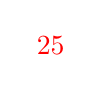
\begin{tikzpicture}
\Tree
[.20
    [.13
    \edge[];
        [.8
        \edge[]; {5}
        \edge[blank]; \node[red]{25};
        ]
    \edge[]; {7}
    ]
    [.17
    \edge[]; {4}
    \edge[]; {2}
    ]
]
\end{tikzpicture}
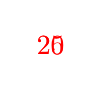
\begin{tikzpicture}
\Tree
[.17
    [.13
    \edge[];
        [.8
        \edge[blank]; \node[red]{20};
        \edge[blank]; \node[red]{25};
        ]
    \edge[]; {7}
    ]
    [.5
    \edge[]; {4}
    \edge[]; {2}
    ]
]
\end{tikzpicture}
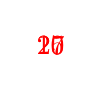
\begin{tikzpicture}
\Tree
[.13
    [.8
    \edge[];
        [.2
        \edge[blank]; \node[red]{20};
        \edge[blank]; \node[red]{25};
        ]
    \edge[]; {7}
    ]
    [.5
    \edge[]; {4}
    \edge[blank]; \node[red]{17};
    ]
]
\end{tikzpicture}
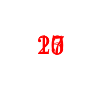
\begin{tikzpicture}
\Tree
[.8
    [.7
    \edge[];
        [.2
        \edge[blank]; \node[red]{20};
        \edge[blank]; \node[red]{25};
        ]
    \edge[]; {4}
    ]
    [.5
    \edge[blank]; \node[red]{13};
    \edge[blank]; \node[red]{17};
    ]
]
\end{tikzpicture}

\vspace{1em}

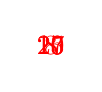
\begin{tikzpicture}
\Tree
[.7
    [.4
    \edge[];
        [.2
        \edge[blank]; \node[red]{20};
        \edge[blank]; \node[red]{25};
        ]
    \edge[blank]; \node[red]{8};
    ]
    [.5
    \edge[blank]; \node[red]{13};
    \edge[blank]; \node[red]{17};
    ]
]
\end{tikzpicture}
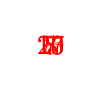
\begin{tikzpicture}
\Tree
[.5
    [.4
    \edge[blank];
        [.\node[red]{7};
        \edge[blank]; \node[red]{20};
        \edge[blank]; \node[red]{25};
        ]
    \edge[blank]; \node[red]{8};
    ]
    [.2
    \edge[blank]; \node[red]{13};
    \edge[blank]; \node[red]{17};
    ]
]
\end{tikzpicture}
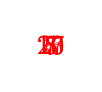
\begin{tikzpicture}
\Tree
[.4
    \edge[];
    [.2
    \edge[blank];
        [.\node[red]{7};
        \edge[blank]; \node[red]{20};
        \edge[blank]; \node[red]{25};
        ]
    \edge[blank]; \node[red]{8};
    ]
    \edge[blank];
    [.\node[red]{5};
    \edge[blank]; \node[red]{13};
    \edge[blank]; \node[red]{17};
    ]
]
\end{tikzpicture}
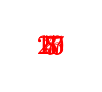
\begin{tikzpicture}
\Tree
[.2
    \edge[blank];
    [.\node[red]{4};
    \edge[blank];
        [.\node[red]{7};
        \edge[blank]; \node[red]{20};
        \edge[blank]; \node[red]{25};
        ]
    \edge[blank]; \node[red]{8};
    ]
    \edge[blank];
    [.\node[red]{5};
    \edge[blank]; \node[red]{13};
    \edge[blank]; \node[red]{17};
    ]
]
\end{tikzpicture}
\end{center}
\end{framed}

\item[6.4-2]{Argue the correctness of \textsc{HeapSort} using the following loop
invariant:
\begin{quote}
At the start of each iteration of the \textbf{for} loop of line 2{--}5, the
subarray $A[1 \dots i]$ is a max-heap containing the $i$ smallest elements of
$A[1 \dots n]$, and the subarray $A[i + 1 \dots n]$ contains the $n - i$ largest
elements of $A[1 \dots n]$, sorted. \vspace{0.5em}
\end{quote}
}

\begin{framed}
We need to show that this invariant is true prior to the first loop iteration,
that each iteration of the loop maintains the invariant, and that the invariant
provides a useful property to show correctness when the loop terminates.

\begin{itemize}
  \item \textbf{Initialization.} Before the \textbf{for} loop, $i = n$ and line
    $1$ assures $A$ is a max-heap. Thus, $A[1, \dots, i] = A$ is a max-heap
    containing the $i$ smallest elements of $A$ and
    $A[i + 1, \dots, n] = \emptyset$ contains the $n - i = 0$ largest elements
    of $A$, sorted.
  \item \textbf{Maintenance.} By the loop invariant, $A[1, \dots, i]$ is
    a max-heap containing the $i$ smallest elements of $A$, which implies that
    $A[1]$ is the $i$th smallest element of $A$. Since $A[i + 1, \dots, n]$
    already contains the $n - i$ largest elements of $A$ in sorted order, after
    exchanging $A[1]$ with $A[i]$, the subarray $A[i, \dots, n]$ now contains
    the $n - i + 1$ largest elements of $A$ in sorted order. Lines 4-5 maintains
    the max-heap property on the subarray $A[1, \dots, i - 1]$ and decrement $i$
    for the next iteration preserves the loop invariant.
  \item \textbf{Termination.} At termination $i = 1$ and the subarray
    $A[2, \dots n]$ contains the $n - 1$ smallest elements of $A$ in sorted
    order, which also implies that $A[1, \dots, n]$ is fully sorted.
\end{itemize}
\end{framed}

\newpage

\item[6.4-3]{What is the running time of \textsc{HeapSort} on an array $A$ of
length $n$ that is already sorted in increasing order? What about decreasing
order?}

\begin{framed}
Since an array that is sorted in increasing order is not a max-heap,
\textsc{Build-Max-Heap} will break that ordering. The \textsc{Build-Max-Heap}
procedure will take $\Theta(n)$ to build the max-heap and the \textbf{for} loop
of lines $2{-}5$ will take $O(n \lg n)$, which gives a total running time of
$\Theta(n) + O(n \lg n) = O(n \lg n)$.

An array sorted in drecreasing order is already a max-heap, but even in that
case \textsc{Build-Max-Heap} will take $\Theta(n)$. Note that, although the
input is sorted in decreasing order, the intent of the algorithm is to sort in
increasing order. In each iteration of the \textbf{for} loop of lines $2{-}5$,
it will exchange $A[1]$ with $A[i]$ and will call \textsc{Max-Heapify} on
$A[1]$. Since $A[1]$ is not anymore the largest element of $A$, each call to
\textsc{Max-Heapify} may cover the entire height of the heap and thus will take
$O(\lg n)$. Thus, the \textbf{for} loop of lines $2{-}5$ will run in
$O(n \lg n)$ and the algorithm will take $\Theta(n) + O(n \lg n) = O(n \lg n)$.
\end{framed}

\item[6.4-4]{Show that the worst-case running time of \textsc{HeapSort} is
$\Omega(n \lg n)$.}

\begin{framed}
The worst-case is when every call to \textsc{Max-Heapify} covers the entire
height of the heap. In that case, \textsc{HeapSort} will take
\[
  \sum_{i = 1}^{n - 1} \floor{\lg i} \le \sum_{i = 1}^{n - 1} \lg i = \lg((n - 1)!) = \Theta((n - 1) \lg (n - 1)) = \Omega(n \lg n).
\]
\end{framed}

\item[6.4-5]{($\star$) Show that when all elements are distinct, the best-case
running time of \textsc{HeapSort} is $\Omega(n \lg n)$.}

\begin{framed}
Proof on (Theorem 1, Page 86):
\begin{quote}
Schaffer, Russel, and Robert Sedgewick. ``The analysis of heapsort.''
\emph{Journal of Algorithms} 15.1 (1993): 76-100.
\end{quote}
\end{framed}

\end{enumerate}

\newpage

{\large Section 6.5 {--} Priority queues}

\begin{enumerate}

\item[6.5{-}1]{Illustrate the operation of \textsc{Heap-Extract-Max}
on the heap $A = \langle 15, 13, 9, 5, 12, 8, 7, 4, 0, 6, 2, 1 \rangle$.}

\begin{framed}
\begin{center}
\begin{tikzpicture}
\Tree
[.15
    [.13
    \edge[];
        [.5
        \edge[]; {4}
        \edge[]; {0}
        ]
    \edge[];
        [.12
        \edge[]; {6}
        \edge[]; {2}
        ]
    ]
    [.9
    \edge[];
        [.8
        \edge[]; {1}
        \edge[blank]; \node[blank]{};
        ]
    \edge[]; {7}
    ]
]
\end{tikzpicture}

\vspace{1em}

\begin{tikzpicture}
\Tree
[.\node[red]{1};
    [.13
    \edge[];
        [.5
        \edge[]; {4}
        \edge[]; {0}
        ]
    \edge[];
        [.12
        \edge[]; {6}
        \edge[]; {2}
        ]
    ]
    [.9
    \edge[]; {8}
    \edge[]; {7}
    ]
]
\end{tikzpicture}
\begin{tikzpicture}
\Tree
[.13
    [.\node[red]{1};
    \edge[];
        [.5
        \edge[]; {4}
        \edge[]; {0}
        ]
    \edge[];
        [.12
        \edge[]; {6}
        \edge[]; {2}
        ]
    ]
    [.9
    \edge[]; {8}
    \edge[]; {7}
    ]
]
\end{tikzpicture}
\begin{tikzpicture}
\Tree
[.13
    [.12
    \edge[];
        [.5
        \edge[]; {4}
        \edge[]; {0}
        ]
    \edge[];
        [.\node[red]{1};
        \edge[]; {6}
        \edge[]; {2}
        ]
    ]
    [.9
    \edge[]; {8}
    \edge[]; {7}
    ]
]
\end{tikzpicture}
\begin{tikzpicture}
\Tree
[.13
    [.12
    \edge[];
        [.5
        \edge[]; {4}
        \edge[]; {0}
        ]
    \edge[];
        [.6
        \edge[]; \node[red]{1};
        \edge[]; {2}
        ]
    ]
    [.9
    \edge[]; {8}
    \edge[]; {7}
    ]
]
\end{tikzpicture}
\end{center}
\end{framed}

\item[6.5{-}2]{Illustrate the operation of \textsc{Max-Heap-Insert}$(A, 10)$
on the heap $A = \langle 15, 13, 9, 5, 12, 8, 7, 4, 0, 6, 2, 1 \rangle$.}

\begin{framed}
\begin{center}
\begin{tikzpicture}
\Tree
[.15
    [.13
    \edge[];
        [.5
        \edge[]; {4}
        \edge[]; {0}
        ]
    \edge[];
        [.12
        \edge[]; {6}
        \edge[]; {2}
        ]
    ]
    [.9
    \edge[];
        [.8
        \edge[]; {1}
        \edge[blank]; \node[blank]{};
        ]
    \edge[]; {7}
    ]
]
\end{tikzpicture}

\vspace{1em}

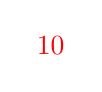
\begin{tikzpicture}
\Tree
[.15
    [.13
    \edge[];
        [.5
        \edge[]; {4}
        \edge[]; {0}
        ]
    \edge[];
        [.12
        \edge[]; {6}
        \edge[]; {2}
        ]
    ]
    [.9
    \edge[];
        [.8
        \edge[]; {1}
        \edge[]; \node[red]{10};
        ]
    \edge[]; {7}
    ]
]
\end{tikzpicture}
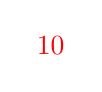
\begin{tikzpicture}
\Tree
[.15
    [.13
    \edge[];
        [.5
        \edge[]; {4}
        \edge[]; {0}
        ]
    \edge[];
        [.12
        \edge[]; {6}
        \edge[]; {2}
        ]
    ]
    [.9
    \edge[];
        [.\node[red]{10};
        \edge[]; {1}
        \edge[]; {8}
        ]
    \edge[]; {7}
    ]
]
\end{tikzpicture}
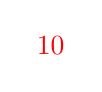
\begin{tikzpicture}
\Tree
[.15
    [.13
    \edge[];
        [.5
        \edge[]; {4}
        \edge[]; {0}
        ]
    \edge[];
        [.12
        \edge[]; {6}
        \edge[]; {2}
        ]
    ]
    [.\node[red]{10};
    \edge[];
        [.9
        \edge[]; {1}
        \edge[]; {8}
        ]
    \edge[]; {7}
    ]
]
\end{tikzpicture}
\end{center}
\end{framed}

\newpage

\item[6.5{-}3]{Write pseudocode for the procedures \textsc{Heap-Minimum},
\textsc{Heap-Extract-Min}, \textsc{Heap-Decrease-Key}, and
\textsc{Min-Heap-Insert} that implement a min-priority queue with a min-heap.}

\begin{framed}
The pseudocodes are stated below.

\begin{algorithm}[H]
\SetAlgoNoEnd\DontPrintSemicolon
\BlankLine
\SetKwFunction{algo}{Heap-Minimum}
\SetKwProg{myalg}{}{}{}
\myalg{\algo{A}}{%
\nl \Return{$A[1]$}\; }
\end{algorithm}

\begin{algorithm}[H]
\SetAlgoNoEnd\DontPrintSemicolon
\BlankLine
\SetKwFunction{algo}{Heap-Extract-Min}
\SetKwProg{myalg}{}{}{}
\myalg{\algo{A}}{%
\nl \If{$A.\text{heap-size} < 1$}{%
\nl \textbf{error} ``heap underflow''\; }
\nl \emph{min} = $A[1]$\;
\nl $A[1] = A[A.\text{\emph{heap-size}}]$\;
\nl $A.\text{\emph{heap-size}} = A.\text{\emph{heap-size}} - 1$\;
\nl \texttt{Min-Heapify}$(A, 1)$\;
\nl \Return{min}\; }
\end{algorithm}

\begin{algorithm}[H]
\SetAlgoNoEnd\DontPrintSemicolon
\BlankLine
\SetKwFunction{algo}{Heap-Decrease-Key}
\SetKwProg{myalg}{}{}{}
\myalg{\algo{A, i, key}}{%
\nl \If{$\text{key} > A[i]$}{%
\nl   \textbf{error} ``new key is larger than current key''\; }
\nl $A[i] = key$\;
\nl \While{$i > 1$ \textbf{and} $A[\texttt{\upshape{Parent}}(i)] > A[i]$}{%
\nl   \upshape{exchange} $A[i]$ \upshape{with} $A[\texttt{Parent}(i)]$\;
\nl   $i = \texttt{Parent}(i)$\; } }
\end{algorithm}

\begin{algorithm}[H]
\SetAlgoNoEnd\DontPrintSemicolon
\BlankLine
\SetKwFunction{algo}{Min-Heap-Insert}
\SetKwProg{myalg}{}{}{}
\myalg{\algo{A, key}}{%
\nl $A.\text{\emph{heap-size}} = A.\text{\emph{heap-size}} + 1$\;
\nl $A[A.\text{\emph{heap-size}}] = +\infty$\;
\nl \texttt{Heap-Decrease-Key}$(A, A.\text{\emph{heap-size}}, key)$\; }
\end{algorithm}
\end{framed}

\item[6.5{-}4]{Why do we bother setting the key of the inserted node to
$-\infty$ in line 2 of \textsc{Max-Heap-Insert} when the next thing we do is
increase its key to the desired value?}

\begin{framed}
Beacause the \textsc{Heap-Increase-Key} procedure requires that the new key is
greater than or equal to the current key.
\end{framed}

\item[6.5{-}5]{Argue the correctness of \textsc{Heap-Increase-Key} using the
folowing loop invariant:
\begin{quote}
At the start of each iteration of the \textbf{while} loop of lines 4-6,
$A[\textsc{Parent}(i)] \ge A[\textsc{Left}(i)]$ and
$A[\textsc{Parent}(i)] \ge A[\textsc{Right}(i)]$, if these nodes exist, and the
subarray $A[1, \dots, A.\text{\emph{heap-size}}]$ satisfies the max-heap
property, except that there may be one violation: $A[i]$ may be larger than
$A[\textsc{Parent}(i)]$.

\end{quote}
You may assume that subarray $A[1, \dots, A.\text{\emph{heap-size}}]$
satisfies the max-heap property at the time \textsc{Heap-Increase-Key} is
called.
}

\begin{framed}
We need to show that this invariant is true prior to the first loop iteration,
that each iteration of the loop maintains the invariant, and that the invariant
provides a useful property to show correctness when the loop terminates.

\begin{itemize}
\item \textbf{Initialization.} Before the \textbf{while} loop, $A$ is
a valid max-heap with a possible change on the value of the element $A[i]$.
Thus, the invariants $A[\textsc{Parent}(i)] \ge A[\textsc{Left}(i)]$ and
$A[\textsc{Parent}(i)] \ge A[\textsc{Right}(i)]$ holds (these values were
not changed before the loop). Since the new value of $A[i]$ is equal or larger
its previous value and its previous value was equal or larger than the value of
its children ($A$ was a max-heap at the time \textsc{Heap-Increse-Key}
was called), the only possible violation on the heap is that $A[i]$ may be
larger than $A[\textsc{Parent}(i)]$, thus the second invariant also holds.
\item \textbf{Maintenance.} By the loop invariant, the only possible violation
is that $A[i]$ may be larger than $A[\textsc{Parent}(i)]$. If there is no
violation ($A[i]$ does not have a parent of $A[i] \le A[\textsc{Parent}(i)]$),
the loop terminates and $A$ is a valid max-heap. If there is a violation on
$A[i]$, the positions of $A[i]$ and $A[\textsc{Parent}(i)]$ are exchanged.
From the loop invariant, before the exchange,
$A[\textsc{Parent}(i)] \ge A[\textsc{Left}(i)]$ and
$A[\textsc{Parent}(i)] \ge A[\textsc{Right}(i)]$, which implies that, after
the exchange, the new $A[i]$ will not violate the max-heap property anymore and
the invariants $A[\textsc{Parent}(i)] \ge A[\textsc{Left}(i)]$ and
$A[\textsc{Parent}(i)] \ge A[\textsc{Right}(i)]$ will remain valid. The only
possible violation after the exchange is that $A[\textsc{Parent}(i)]$ may be
larger than $A[\textsc{Parent}(\textsc{Parent}(i))]$, but setting
$i = \textsc{Parent}(i)$ preserves the loop invariant for the next iteration.
\item \textbf{Termination.} At termination, either $i = 1$ or
$A[i] \le A[\textsc{Parent}(i)]$. In both cases, $A[i]$ is not larger than
$A[\textsc{Parent}(i)]$, which implies that $A$ is a valid max-heap.
\end{itemize}
\end{framed}

\item[6.5{-}6]{Each exchange operation on line 5 of \textsc{Heap-Increase-Key}
typically requires three assignments. Show how to use the idea of the inner
loop of \textsc{Insertion-Sort} to reduce the three assignments down to just one
assignment.}

\begin{framed}
The updated pseudocode is stated below.

\begin{algorithm}[H]
\SetAlgoNoEnd\DontPrintSemicolon
\BlankLine
\SetKwFunction{algo}{Heap-Increase-Key}
\SetKwProg{myalg}{}{}{}
\myalg{\algo{A, i, key}}{%
\nl \If{$\text{key} < A[i]$}{%
\nl   \textbf{error} ``new key is smaller than current key''\; }
\nl \While{$i > 1$ \textbf{and} $A[\texttt{\upshape{Parent}}(i)] < key$}{%
\nl   $A[i] = A[\texttt{Parent}(i)]$\;
\nl   $i = \texttt{Parent}(i)$\; }
\nl $A[i] = key$\; }
\end{algorithm}
\end{framed}

\item[6.5{-}7]{Show how to implement a first-in, first-out queue with a priority
queue. Show how to implement a stack with a priority queue. (Queues and stacks
are defined in Section 10.1.)}

\begin{framed}
A first-in, first-out queue can be implemented using a min-priority-queue, in
such a way that each heap element is a tuple (key, handle) and the key of a new
element is greater than the key of the current elements. The
\textsc{Extract-Min} operation will always return the oldest element (minimum
key value) and the \textsc{Insert} operation will keep the min-heap property.
A stack can be implemented similarly, but with a max-priority-heap instead of
a min-priority-heap.
\end{framed}

\item[6.5{-}8]{The operation \textsc{Heap-Delete}$(A, i)$ deletes the item in
node $i$ from heap $A$. Give an implementation of \textsc{Heap-Delete} that runs
in $O(\lg n)$ time for an $n$-element max-heap.}

\begin{framed}
The pseudocode is stated below.

\begin{algorithm}[H]
\SetAlgoNoEnd\DontPrintSemicolon
\BlankLine
\SetKwFunction{algo}{Heap-Delete}
\SetKwProg{myalg}{}{}{}
\myalg{\algo{A, i}}{%
\nl $A[i] = A[\text{\emph{heap-size}}]$\;
\nl $A.\text{\emph{heap-size}} = A.\text{\emph{heap-size}} - 1$\;
\nl \texttt{Max-Heapify}$(A, i)$\; }
\end{algorithm}
\end{framed}

\item[6.5{-}9]{Give an $O(n \lg k)$-time algorithm to merge $k$ sorted lists
into one sorted list, where $n$ is the total number of elements in all the input
lists. (Hint: Use a min-heap for $k$-way merging.)}

\begin{framed}
Let $T$ denote the final sorted list and $S_i$ the $i$th input list. The
pseudocode is stated below.

\begin{algorithm}[H]
\SetAlgoNoEnd\DontPrintSemicolon
\BlankLine
\SetKwFunction{algo}{Merge-Lists-Min-Heap}
\SetKwProg{myalg}{}{}{}
\myalg{\algo{$S_1, S_2, \dots, S_k$}}{%
\nl Let $T$ be a list\;
\nl Let $H$ be a min-heap of tuples in the form $(key, j)$\;
\nl \For{$i = 1$ \KwTo $k$}{%
\nl   $\texttt{Insert}(H, (S_i[1], i))$\;
\nl   $p_i = 2$\; }
\nl \While{$H.\text{heap-size} > 0$}{%
\nl   $(key, j) = \texttt{Extract-Min}(H)$\;
\nl   add $key$ to $T$\;
\nl   \If{$p_j \le S_j.\text{length}$}{%
\nl     $\texttt{Insert}(H, (S_j[p_j], j))$\;
\nl     $p_j = p_j + 1$\; } }
\nl \Return{T}\; }
\end{algorithm}

The \textbf{for} loop of lines 3{-}5 runs in $O(k \lg k)$. The \textbf{while}
loop of lines 6{-}11 will iterate $n$ times and each iteration takes $O(\lg k)$.
Since $n \ge k$, the algorithm runs in $O(n \lg k)$.
\end{framed}

\end{enumerate}

\newpage

{\large Problems}

\begin{enumerate}


\item[6{-}1]{\textbf{\emph{Building a heap using insertion}}\\
We can build a heap by repeatedly calling \textsc{Max-Heap-Insert} to insert
the elements into the heap. Consider the following variation on the
\textsc{Build-Max-Heap} procedure:

\begin{algorithm}[H]
\SetAlgoNoEnd\DontPrintSemicolon
\BlankLine
\SetKwFunction{algo}{Build-Max-Heap'}
\SetKwProg{myalg}{}{}{}
\myalg{\algo{A}}{%
\nl $A.\text{\emph{heap-size}} = 1$\;
\nl \For{$i = 2$ \KwTo $A.\text{length}$}{%
\nl   $\textsc{Max-Heap-Insert}(A, A[i])$\; } }
\end{algorithm}

\begin{enumerate}
\item[\textbf{a.}]{Do the procedures \textsc{Build-Max-Heap} and
\textsc{Build-Max-Heap\texttt{'}} always create the same heap when run on the
same input array? Prove that they do, or provide a counterexample.}
\item[\textbf{b.}]{Show that in the worst-case,
\textsc{Build-Max-Heap\texttt{'}} requires $\Theta(n \lg n)$ time to build an
$n$-element heap.}
\end{enumerate}

}

\begin{framed}
\begin{enumerate}

\item No. Consider the array $A = [1, 2, 3]$. \textsc{Build-Max-Heap}$(A)$ will
create the heap
\begin{center}
\begin{tikzpicture}
\Tree
  [.\node[red]{1};
  \edge[]; {2}
  \edge[]; {3}
]
\end{tikzpicture}
\begin{tikzpicture}
\Tree
  [.3
  \edge[]; {2}
  \edge[]; {1}
]
\end{tikzpicture}
\end{center}

while \textsc{Build-Max-Heap\texttt{'}}$(A)$ will create the heap

\begin{center}
\begin{tikzpicture}
\Tree
  [.1
  \edge[]; \node[red]{2};
  \edge[]; {3}
]
\end{tikzpicture}
\begin{tikzpicture}
\Tree
  [.2
  \edge[]; {1}
  \edge[]; \node[red]{3};
]
\end{tikzpicture}
\begin{tikzpicture}
\Tree
  [.3
  \edge[]; {1}
  \edge[]; {2}
]
\end{tikzpicture}
\end{center}

\item Let $A$ be the input array. The worst-case occurs when there is an integer
$k$ such that $n = A.\text{\emph{length}} = 2^k - 1$ (that is, the elements of
$A$ forms a complete binary tree) and each call to \textsc{Max-Heap-Insert}
covers the entire height of the heap (occurs when $A$ is sorted). Since any heap
has $\ceil{n/2}$ leaves, the last $\ceil{n/2}$ elements of $A$ will be the
leaves of the final heap. Note that, at the time \textsc{Max-Heap-Insert} is
called on these last $\ceil{n/2}$ nodes, the height of the heap will be
$\floor{\lg n}$. Thus, considering only the last $\ceil{n/2}$ calls to
$\textsc{Max-Heap-Insert}$, the algorithm will take $\ceil{n/2} \cdot
\Theta(\floor{\lg n}) = \Theta(n \lg n)$, which implies that the worst-case
of \textsc{Build-Max-Heap\texttt{'}} runs in $\Omega(n \lg n)$. Also, note
that there will be exactly $n - 1$ calls to \textsc{Max-Heap-Insert} and
each call takes $O(\floor{\lg n})$. Thus, the worst-case of
\textsc{Build-Max-Heap\texttt{'}} runs in $\Theta(n \lg n)$.
\end{enumerate}
\end{framed}

\newpage

\item[6{-}2]{\textbf{\emph{Analysis of d-ary heaps}}\\
A \textbf{\emph{d-ary}} heap is like a binary heap, but (with one possible
exception) non-leaf nodes have $d$ children instead of 2 children.
\begin{enumerate}
\item[\textbf{a.}] How would you represent a $d$-ary heap in an array?
\item[\textbf{b.}] What is the height of a $d$-ary heap of $n$ elements in terms
of $n$ and $d$?
\item[\textbf{c.}] Give an efficient implementation of \textsc{Extract-Max} in
a $d$-ary max-heap. Analyze its running time in terms of $d$ and $n$.
\item[\textbf{d.}] Give an efficient implementation of \textsc{Insert} in
a $d$-ary max-heap. Analyze its running time in terms of $d$ and $n$.
\item[\textbf{e.}] Give an efficient implementation of
\textsc{Increase-Key}$(A, i, k)$, which flags an error if $k < A[i]$, but
otherwise sets $A[i] = k$ and then updates the $d$-ary max-heap structure
appropriately. Analyze its running time in terms of $d$ and $n$.
\end{enumerate}
}

\begin{framed}
\begin{enumerate}
\item The root occupies the first $d^0 = 1$ positions of the array, its
children occupies the next $d^1 = d$ positions of the array, and so on until
the bottom level. That way, the parent of a node with index $i$ will be at
position
\[
  \Bigl\lfloor{\frac{i - (d - 2)}{d}}\Bigr\rfloor
  = \Bigl\lfloor{\frac{i - d + 2}{d}}\Bigr\rfloor,
\]
and its $j$th children will be at position
\[
  di - (d - j) + 1 = di - d + j + 1 = d (i - 1) + j + 1.
\]

\item $h = \floor{\log_d n}$.

\item The only major modification is the \textsc{Max-Heapify} procedure. The
pseudocode is stated below.

\begin{algorithm}[H]
\SetAlgoNoEnd\DontPrintSemicolon
\BlankLine
\SetKwFunction{algo}{Child-D-Ary}
\SetKwProg{myalg}{}{}{}
\myalg{\algo{d, i, j}}{%
\nl \Return{$d (i - 1) + j + 1$}\; }
\end{algorithm}

\begin{algorithm}[H]
\SetAlgoNoEnd\DontPrintSemicolon
\BlankLine
\SetKwFunction{algo}{Extract-Max-D-Ary}
\SetKwProg{myalg}{}{}{}
\myalg{\algo{A, d}}{%
\nl \If{$A.\text{heap-size} < 1$}{%
\nl   \textbf{error} ``heap underflow''\; }
\nl $\text{\emph{max}} = A[1]$\;
\nl $A.\text{\emph{heap-size}} = A.\text{\emph{heap-size}} - 1$\;
\nl $\texttt{Max-Heapify-D-Ary}(A, d, 1)$\;
\nl \Return{\text{max}}\; }
\end{algorithm}

\begin{algorithm}[H]
\SetAlgoNoEnd\DontPrintSemicolon
\BlankLine
\SetKwFunction{algo}{Max-Heapify-D-Ary}
\SetKwProg{myalg}{}{}{}
\myalg{\algo{A, d, i}}{%
\nl $\text{\emph{largest}} = i$\;
\nl \For{$j = 1$ \KwTo $d$}{%
\nl   $\text{\emph{child-j}} = \texttt{Child}(d, i, j)$\;
\nl   \If{$\text{child-j} > A.\text{heap-size}$}{%
\nl     break\; }
\nl   \If{$A[\text{child-j}] > A[\text{largest}]$}{%
\nl     $\text{\emph{largest}} = \text{\emph{child-j}}$\; } }
\nl \If{$\text{largest} \neq i$}{%
\nl   exchange $A[i]$ with $A[\text{\emph{largest}}]$\;
\nl   $\texttt{Max-Heapify-D-Ary}(A, d, \text{\emph{largest}})$\; } }
\end{algorithm}

In the worst-case, \textsc{Max-Heapify-D-Ary} covers the height of the heap
(which is $\log_d n$).  Since each recursive call takes $O(d)$,
\textsc{Max-Heapify-D-Ary} runs in $O(d \log_d n)$. The running time of
\textsc{Extract-Max-D-Ary} is also $O(d \log_d n)$, since it performs a constant
amount of work on top of \textsc{Max-Heapify-D-Ary}.

\item The $\textsc{Max-Heap-Insert}$ procedure given in the text book also works
for a $d$-ary heap. The only modification is to use \textsc{Parent-D-Ary}
instead of \textsc{Parent} in the \textsc{Heap-Increase-Key} subroutine. In the
worst case, it will cover the height of the tree. Thus, the running time is
$O(\log_d n)$.

\item The $\textsc{Heap-Increase-Key}$ procedure given in the text book also
works for a $d$-ary heap. The only modification is to use \textsc{Parent-D-Ary}
instead of \textsc{Parent}. In the worst case, it will cover the height of the
tree. Thus, the running time is $O(\log_d n)$.
\end{enumerate}
\end{framed}

\newpage

\item[6{-}3]{\textbf{\emph{Young tableaus}}\\
An $m \times n$ \textbf{\emph{Young tableau}} is an $m \times n$ matrix such
that the entries of each row are in sorted order from left to right and the
entries of each column are in sorted order from top to bottom. Some of the
entries of a Young tableau may be $\infty$, which we treat as nonexistent
elements. Thus, a Young tableau can be used to hold $r \le mn$ finite numbers.
\begin{enumerate}
\item[\textbf{a.}] Draw a $4 \times 4$ Young tableau containing the elements
$\{9, 16, 3, 2, 4, 8, 5, 14, 12\}$.
\item[\textbf{b.}] Argue that an $m \times n$ Young tableau $Y$ is empty if
$Y[1, 1] = \infty$. Argue that $Y$ is full (contains $mn$ elements) if
$Y[m, n] < \infty$.
\item[\textbf{c.}] Give an algorithm to implement \textsc{Extract-Min} on
a non-empty $m \times n$ Young tableau that runs in $O(m + n)$ time. Your
algorithm should use a recursive subroutine that solves an $m \times n$ problem
by recursively solving either an $(m - 1) \times n$ or an $m \times (n - 1)$
subproblem. (Hint: Think about \textsc{Max-Heapify}.) Define $T(p)$, where
$p = m + n$, to be the maximum running time of \textsc{Extract-Min} on any
$m \times n$ Young tableau. Give and solve a recurrence for $T(p)$ that yields
the $O(m + n)$ time bound.
\item[\textbf{d.}] Show how to insert a new element into a nonfull $m \times n$
Young tableau in $O(m + n)$ time.
\item[\textbf{e.}] Using no other sorting method as a subroutine, show how to
use an $n \times n$ Young tableau to sort $n^2$ numbers in $O(n^3)$ time.
\item[\textbf{f.}] Give an $O(m + n)$-time algorithm to determine whether
a given number is stored in a given $m \times n$ Young tableau.
\end{enumerate}
}

\begin{framed}
\begin{enumerate}
\item Here it is:

\begin{center}
\begin{tabular}{cccc}
  2 & 3 & 4 & 5\\
  8 & 9 & 12 & 14\\
  16 & $\infty$ & $\infty$ & $\infty$\\
  $\infty$ & $\infty$ & $\infty$ & $\infty$
\end{tabular}
\end{center}

\item From the definition of a Young tableau, we have
\[
  Y[1, 1] \le Y[i, j]\;\Forall i, j,
\]
which implies
\[
  Y[1, 1] = \infty \rightarrow Y[i, j] = \infty\;\Forall i, j.
\]
Thus, $Y$ is full of $\infty$ and is therefore empty.

From the definition of a Young tableau, we have
\[
  Y[m, n] \ge Y[i, j]\;\Forall i, j,
\]
which implies
\[
  Y[m, n] < \infty \rightarrow Y[i, j] < \infty\;\Forall i, j.
\]
Thus, $Y$ does not have any $\infty$ and is therefore full.

\item The pseudocode is stated below.

\begin{algorithm}[H]
\SetAlgoNoEnd\DontPrintSemicolon
\BlankLine
\SetKwFunction{algo}{Extract-Min}
\SetKwProg{myalg}{}{}{}
\myalg{\algo{Y}}{%
\nl $\text{\emph{min}} = Y[1, 1]$\;
\nl \If{$\text{min} == \infty$}{%
\nl    \textbf{error} ``tableau underflow''\; }
\nl $Y[1, 1] = \infty$\;
\nl $\texttt{Min-Tableauify}(Y, 1, 1)$\;
\nl \Return{min}\; }
\end{algorithm}

\begin{algorithm}[H]
\SetAlgoNoEnd\DontPrintSemicolon
\BlankLine
\SetKwFunction{algo}{Min-Tableauify}
\SetKwProg{myalg}{}{}{}
\myalg{\algo{Y, i, j}}{%
\nl $\text{\emph{smallest-i}} = i$\;
\nl $\text{\emph{smallest-j}} = j$\;
\nl \If{$i + 1 \le Y.\text{rows}$ \textbf{\upshape{and}} $Y[i + 1, j] < Y[\text{smallest-i}, \text{smallest-j}]$}{%
\nl   $\text{\emph{smallest-i}} = i + 1$\; }
\nl \If{$j + 1 \le Y.\text{cols}$ \textbf{\upshape{and}} $Y[i, j + 1] < Y[\text{smallest-i}, \text{smallest-j}]$}{%
\nl   $\text{\emph{smallest-i}} = i$\;
\nl   $\text{\emph{smallest-j}} = j + 1$\; }
\nl \If{$i \neq \text{smallest-i}$ \textbf{\upshape{or}} $j \neq \text{smallest-j}$}{%
\nl   $Y[i, j] = Y[\text{\emph{smallest-i}}, \text{\emph{smallest-j}}]$\;
\nl   $Y[\text{\emph{smallest-i}}, \text{\emph{smallest-j}}] = \infty$\;
\nl   $\texttt{Min-Tableauify}(Y, \text{\emph{smallest-i}}, \text{\emph{smallest-j}})$\; } }
\end{algorithm}

The algorithm has the recurrence $T(p) \le T(p - 1) + \Theta(1) = O(p) + O(m + n)$.

\item The pseudocode is stated below.

\begin{algorithm}[H]
\SetAlgoNoEnd\DontPrintSemicolon
\BlankLine
\SetKwFunction{algo}{Tableau-Insert}
\SetKwProg{myalg}{}{}{}
\myalg{\algo{Y, key}}{%
\nl $i = Y.\text{\emph{rows}}$\;
\nl $j = Y.\text{\emph{cols}}$\;
\nl \If{$Y[i, j] == \infty$}{%
\nl   \textbf{error} ``tableau overflow''\; }
\nl $Y[i, j] = \text{\emph{key}}$\;
\nl \While{$i > 1$ \textbf{\upshape{or}} $j > 1$}{%
\nl   \If{$i > 1$ \textbf{\upshape{and}} $Y[i, j] < Y[i - 1, j]$}{%
\nl     exchange $Y[i, j]$ with $Y[i - 1, j]$\;
\nl     $i = i - 1$\; }
\nl   \ElseIf{$j > 1$ \textbf{\upshape{and}} $Y[i, j] < Y[i, j - 1]$}{%
\nl     exchange $Y[i, j]$ with $Y[i, j - 1]$\;
\nl     $j = j - 1$\; }
\nl   \Else{%
\nl     break\; } } }
\end{algorithm}

We first set the element to the position $A[m, n]$ and move it upwards and/or
leftwards until we find a valid position. The running time is $O(m + n)$

\item The pseudocode is stated below.

\begin{algorithm}[H]
\SetAlgoNoEnd\DontPrintSemicolon
\BlankLine
\SetKwFunction{algo}{Build-Young-Tableau}
\SetKwProg{myalg}{}{}{}
\myalg{\algo{A}}{%
\nl $n = \sqrt{A.\text{\emph{length}}}$\;
\nl Let $Y$ be an $n \times n$ array\;
\nl \For{$i = 1$ \KwTo $A.\text{\emph{length}}$}{%
\nl   \texttt{Tableau-Insert}$(Y, A[i])$\; }
\nl \Return{$Y$}\; }
\end{algorithm}

\begin{algorithm}[H]
\SetAlgoNoEnd\DontPrintSemicolon
\BlankLine
\SetKwFunction{algo}{Tableausort}
\SetKwProg{myalg}{}{}{}
\myalg{\algo{A}}{%
\nl $Y = \textsc{Build-Young-Tableau}(A)$\;
\nl \For{$i = 1$ \KwTo $A.\text{length}$}{%
\nl   $A[i] = \texttt{Extract-Min}(Y)$\; } }
\end{algorithm}

The \textsc{Build-Young-Tableau} procedure runs in
$n^2 \cdot O(n + n) = O(n^3)$. Each call to \textsc{Min-Tableauify} runs in
$O(n + n) = O(n)$. Thus, the algorithm runs in
$O(n^3) + n^2 \cdot O(n) = O(n^3)$.

\item The pseudocode is stated below.

\begin{algorithm}[H]
\SetAlgoNoEnd\DontPrintSemicolon
\BlankLine
\SetKwFunction{algo}{Tableau-Find}
\SetKwProg{myalg}{}{}{}
\myalg{\algo{Y, key}}{%
\nl $i = Y.\text{\emph{rows}}$\;
\nl $j = 1$\;
\nl \While{$i \ge 1$ \textbf{\upshape{and}} $j \le Y.\text{cols}$}{%
\nl   \If{$Y[i, j] == \text{\emph{key}}$}{%
\nl     \Return{\texttt{\upshape{True}}}\; }
\nl   \ElseIf{$Y[i, j] \le Y[i - 1, j]$}{%
\nl     $i = i - 1$\; }
\nl   \ElseIf{$Y[i, j] \ge Y[i, j + 1]$}{%
\nl     $j = j + 1$\; }
\nl   \Else{%
\nl     break\; }
\nl \Return{\texttt{\upshape{False}}}\; } }
\end{algorithm}

\end{enumerate}
\end{framed}

\end{enumerate}
